\chapter{Introduction}\label{chapter-introduction}
\lhead{Chapter 1. \emph{Introduction}}
\section{Introduction}\label{section-introduction}
Intel System on a Chip (\gls{soc}) \cite{intel-soc} features a new set of Intel Uncore Intellectual Property (\gls{ip}) for every generation.
Section \ref{section-introduction} covers the introduction and overview of BIOS, UEFI and it's role and major components - \say{Advanced Configuration and Power Interface (\gls{acpi})}, \say{Peripheral Component Interconnect Express (\gls{pcie})} and Graphics Controller. Section \ref{section-design} describes the design of UEFI and the boot phases in detail. The study of the BIOS binary structure and mapping of each components byte and alignment is described in Section \ref{section-architecture}. Proposed work to reducing the process of build iteration described in Section \ref{section-proposed-work}. 

\subsection{Uncore \gls{ip}}
The Uncore encompasses system agent (SA), memory and Uncore agents such as graphics controller, display controller, memory controller and Input Output (IO).The Uncore IPs are \say{Peripheral Component Interface Express (\gls{pcie})}, \say{Graphics Processing Engine (GPE)}, Thunderbolt, Imaging Processing Agent (IPU), \say{North Peak (NPK)}, \say{Virtualization Technology for directed-IO (Vt-d)}, Volume Management Device (VMD).

PCI Express abbreviated as \gls{pci} or \gls{pcie}, is designed to replace the older PCI standards. A data communicating system is highly-developed via PCIe for use the transfer data between the host and the peripheral devices. Intel developed the hardware interface which allows the connection among the external peripherals to a computer called Thunderbolt. This interface not only has \say{PCI Express (PCIe)} and DisplayPort (DP) combined into two serial signals but additionally provides DC power also, bundled in just one cable.
\say{Graphics Processing Engine (GPE)}, \say{Integrated graphics}, \say{shared graphics solutions}, \say{integrated graphics processors (IGP)} or \say{unified memory architecture(UMA)} utilize a portion of a memory of computer system instead of having dedicated graphics memory.
GPEs can be integrated onto the motherboard as part of the chipset. Guest virtual machines use \say{Virtual Technology for Directed-IO (Vt-d)}, an \say{input/output memory management unit(IOMMU)}, to directly use peripheral devices, such as hard-drive controllers, accelerated graphics cards and Ethernet, through interrupt remapping.

\subsection{Legacy \gls{bios} and \gls{uefi}}

\paragraph{\gls{bios}} is the governing reference which specifies a firmware interface.

"Legacy" (as in Legacy \gls{bios}) -  in terms of firmware specifications it refers to an older, broadly used specification. Major responsibility of \gls{bios} is to initiate the support for hardware devices, loading and commencing an \gls{os}. When the system boots, the BIOS initializes and identifies every connected system devices including keyboard, mouse, hard disk drive, solid state drive, video display card and other hardware followed by locating software stored on a boot device i.e. a hard disk or removable storage such as USB or CD/DVD and loads and executes that software, transferring control of the system to it. This flow of actions is also known as "booting" or "boot strapping".

Table \ref{table:legacy-bios-vs-uefi} overviews of comparisons of UEFI with legacy BIOS.

\begin{table}
  \centering
  \renewcommand{\arraystretch}{2}
  \caption{Comparison of Legacy BIOS and UEFI}\label{table:legacy-bios-vs-uefi}
  \begin{tabular}{l | p{5cm} | p{5cm}}
    & Legacy BIOS & EFI
    \\ \hline \hline
    Programming Language used & Assembly Language & C Language ($ 99\% $)
    \\ \hline
    Resources & Interrupt Hardcode Memory Access hardcore Input/Output Access & Divers, Handlers and Protocols
    \\ \hline
    Processor Type & $ x86 $ $ 16-bit $ & CPU Protects Mode
    \\ \hline
    Expand & Interrupt through hook & Driver to be loaded
    \\ \hline
    OS Communication Bridge & via ACPI & through runtime driver
    \\ \hline
    $ 3^{rd} $ Party ISV \& \gls{ihv} & Support Bas & Ease of Support and for Cross-Platforms
    \\ \hline
  \end{tabular}
\end{table}

\subsubsection{Background of Legacy \gls{bios}}
In 1980s, IBM developed the personal computer with a 16-bit BIOS with the aim of ending the BIOS after the first 250,000 products. Legacy BIOS is based upon Intel’s original 16-bit architecture, ordinarily referred to as "8086" architecture. And as technology advanced, Intel extended that 8086 architecture from 16 to 32-bit. Legacy BIOS is able to run different \gls{os} very well irrespective if the system is IBM or not. Additionally, Legacy BIOS also has a defined OS-independent interface for hardware that enables interrupts to communicate with keyboard, disk and video services along with the BIOS ROM loader and bootstrap loader, to name a few.

Use of legacy BIOS is diminishing and is expected to be phased out in new systems by the year 2020.

\subsubsection{Limitations of legacy BIOS}
With progress in technologies, the BIOS implementations were also updated with many new configuration and power management technologies and added support for many generations of Intel® architecture hardware. Although a few of limitations namely, upper memory block (UMB) dependencies, PC AT hardware dependencies, 1 MB addressable space and 16-bit addressing mode persisted throughout the years. The need to integrate libraries of third-party firmware modules into a single platform solution across multiple product lines and ensuring quality of individual firmware modules arises in the industries. The existing market demands to overcome inherent limitations lead towards development of a fresh BIOS architecture which is introduced in market as The UEFI specifications.

One major problem with existing BIOS implementations is that since they are highly customized for a specific motherboard, there maintenance is difficult. A lot of effort is required in significant porting, integration, testing and debug work of changes in component modules. The UEFI architecture is designed to considering these limitations and to resolve them.


\subsection{Unified Extensible Firmware Interface (\gls{uefi})}
\gls{uefi} is a replacement for legacy BIOS to act as the interface between a operating system and its platform firmware streamlining the booting process. It offers a rich extensible pre-OS environment with advanced boot and runtime services, replacing most BIOS functions. Unified Extensible Firmware Interface (UEFI) is grounded in Intel’s initial Extensible Firmware Interface (EFI) specification 1.10, which defines a software interface providing linking to an operating system and platform firmware. It has intrinsic networking capabilities,  is designed to work with multi-processors (MP) system and also allows users to execute applications on a command line interface.

\begin{figure}[h]
	\centering
	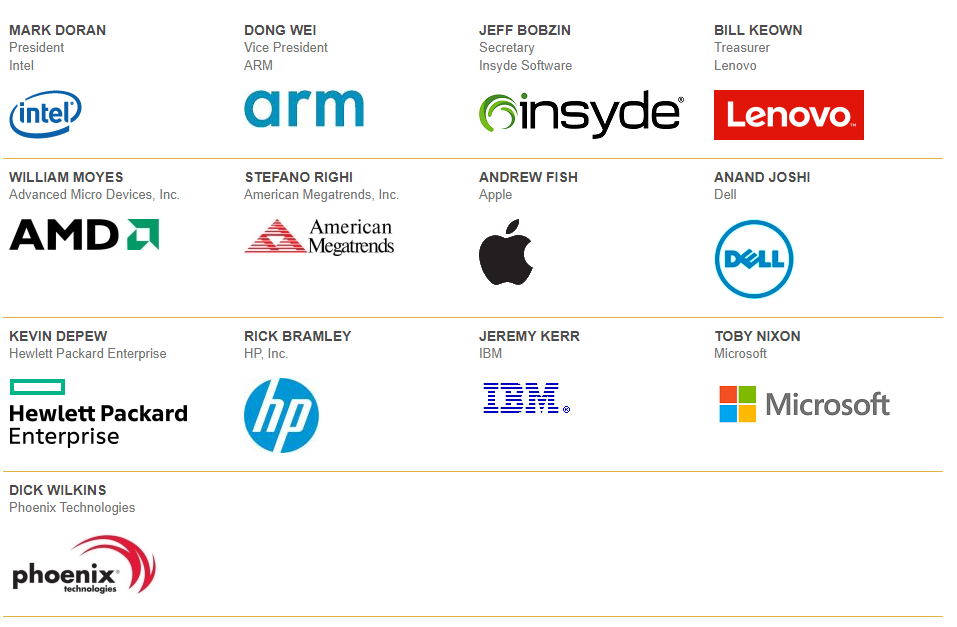
\includegraphics[width=\linewidth]{uefi_board_of_directors}
	\caption{Board of Directors of UEFI Forum \cite{uefi-board-of-directors}}\label{fig:introduction-uefi-board-of-directors}
\end{figure}

The UEFI Forum board of directors consists of representatives from 11 industry leaders as described in Figure \ref{fig:introduction-uefi-board-of-directors}. These organizations work to ensure that the UEFI specifications meet industry needs.

UEFI uses a different interface for runtime services and boot services but UEFI does not specify how "Power On Self Test" (POST) and Setup are implemented those are BIOS’ primary functions.

\subsubsection{\gls{uefi} Driver Model Extension}
Boot devices are accessible via a set of protocol interfaces. The UEFI Driver Model provides a replacement for PC-AT-style option ROMs.

The UEFI Driver Model was not designed to replace the high-performance OS specific drivers but to access boot devices in the pre-boot environment, to support the execution of modular pieces of code, also known as drivers.These drivers control hardware buses and devices on the platform, and also they may provide some software-derived, platform specific service. The information required by the driver developers for implementing combination of bus drivers which boot an UEFI-complaint OS are included in the UEFI Driver Model.

Thus the UEFI Driver Model is designed to be generic.The UEFI Specification describes how to write USB bus drivers, USB device drivers, PCI device drivers, PCI bus drivers and SCSI drivers.
Additional details are provided that allow UEFI drivers to be stashed within PCI option ROMs along with maintaining the compatibility with legacy option ROM images.

The UEFI Specification is designed keeping in mind the goal of having compact driver images. However to facilitate support for multiple processor architectures, a driver object file for each architecture is required to be included leading to a space issue. To resolve this issue, UEFI defines EFI Byte Code Virtual Machine. Every driver file is compiled into just a single EFI Byte Code object which is run by an UEFI Byte Code Interpreter included in the UEFI Specification complaint firmware. Another very common method to resolve this issue is compression. The UEFI specification defined compression and decompression algorithms which may be used to reduce the size of UEFI Drivers.

This information can used by OEMs, \gls{ihv}s, OSVs, and firmware vendors for developing drivers that produce standard protocol interfaces, and operating system loaders which could be utilized to boot UEFI compliant OS.

\subsubsection{\gls{uefi}'s Role in boot process}

During the boot process, UEFI speaks to the operating system loader and acts as the interface linking the operating system and the BIOS.

The \verb|PC-AT| boot environment is challenging to innovate as each new firmware capability requires firmware developers to craft more complex solutions, often requiring OS developers to perform manipulation for their boot code. Since this is a time-consuming process and also required investment of resources, the UEFI specification undertakes it as a primary goal to overcome this issue.


\subsection{Advanced Configuration and Power Interface (\gls{acpi})}
The ACPI Component Architecture (ACPICA) defines and implements a group of software
components that together create an implementation of the ACPI specification. A major goal of the
architecture is to isolate all operating system dependencies to a relatively small translation or
conversion layer (the OS Services Layer) so that the bulk of the ACPICA code is independent of
any individual operating system. Therefore, hosting the ACPICA code on new operating systems
requires no source changes within the ACPICA code itself.

The components of the architecture include:
\begin{itemize}
	\item An OS-independent, kernel-resident ACPICA Subsystem component that provides the fundamental ACPI services such as the AML interpreter and namespace management.
	\item An OS-dependent OS Services Layer for each host operating system to provide OS support for the OS-independent ACPICA Subsystem.
	\item An ASL compiler-disassembler for translating ASL code to AML byte code and for disassembling existing binary ACPI tables back to ASL source code.
	\item Several ACPI utilities for executing the interpreter in ring 3 user space, extracting binary ACPI tables from the output of the ACPI Dump utility, and translating the ACPICA source	code to Linux/Unix format.
\end{itemize}

In Figure \ref{fig:introduction-acpi-component-architecture}, the ACPICA subsystem is shown in relation to the host operating system, device driver, OSPM software, and the ACPI hardware

\begin{figure}[h]
	\centering
	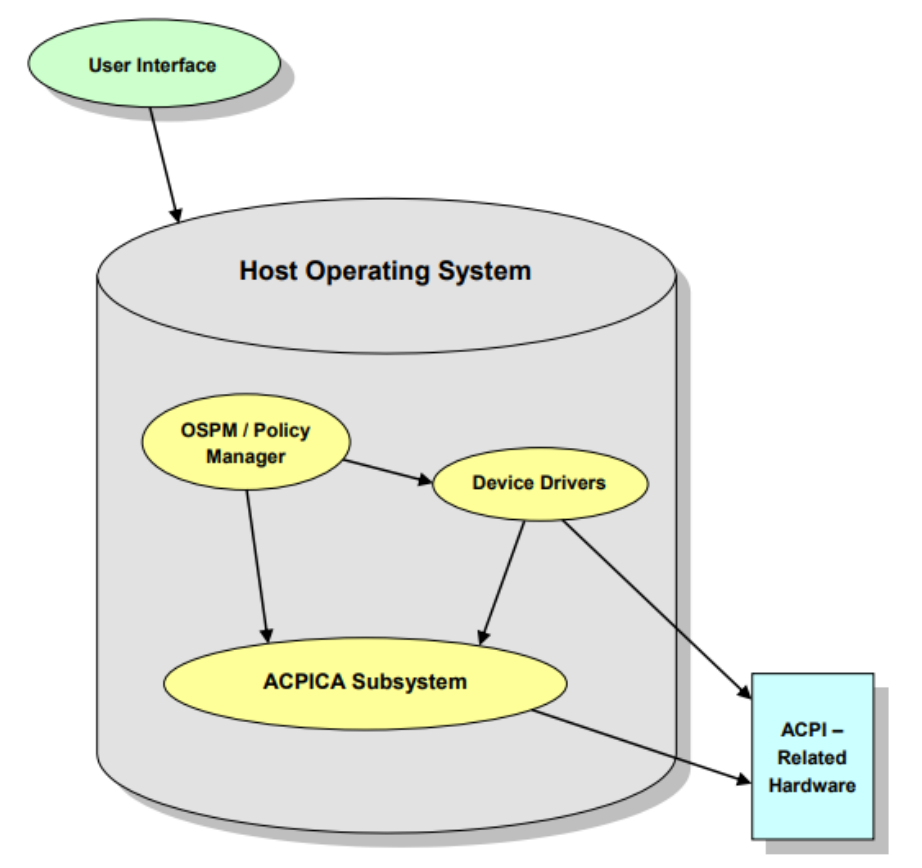
\includegraphics[width=0.7\linewidth]{introduction/acpi-component-architecture}
	\caption{The \gls{acpi} Component Architecture}\label{fig:introduction-acpi-component-architecture}
\end{figure}

\subsubsection{Overview of ACPICA Subsystem}
The ACPICA Subsystem implements the low level or fundamental aspects of the ACPI
specification. Included are an AML parser/interpreter, ACPI namespace management, ACPI table
and device support, and event handling. Since the ACPICA subsystem provides low-level system
services, it also requires low-level operating system services such as memory management,
synchronization, scheduling, and I/O.

To allow the ACPICA Subsystem to easily interface to any operating system that provides such
services, an Operating System Services Layer translates ACPICA-to-OS requests into the system
calls provided by the host operating system. The OS Services Layer is the only component of the
ACPICA that contains code that is specific to a host operating system.

Thus, the ACPICA Subsystem consists of two major software components:
\begin{itemize}
	\item The basic kernel-resident ACPICA Subsystem provides the fundamental ACPI services	that are independent of any particular operating system.
	\item The OS Services Layer (OSL) provides the conversion layer that interfaces the OS independent ACPICA Subsystem to a host operating system.
\end{itemize}

When combined into a single static or loadable software module such as a device driver or
kernel subsystem, these two major components form the ACPICA Subsystem. Throughout this
document, the term "ACPICA Subsystem" refers to the combination of the OS-independent
ACPICA Subsystem with an OS Services Layer components combined into a single module,
driver, or load unit.

\subsubsection{OS-independent ACPICA Subsystem}
The OS-independent ACPICA Subsystem supplies the major building blocks or subcomponents that are required for all ACPI implementations — including an AML interpreter, a namespace manager, ACPI event and resource management, and ACPI hardware support.

One of the goals of the ACPICA Subsystem is to provide an abstraction level high enough such
that the host operating system does not need to understand or know about the very low-level ACPI
details. For example, all AML code is hidden from the host. Also, the details of the ACPI hardware
are abstracted to higher-level software interfaces.

The ACPICA Subsystem implementation makes no assumptions about the host operating system or environment. The only way it can request operating system services is via interfaces provided by the OS Services Layer.

The primary user of the services provided by the ACPICA Subsystem are the host OS device drivers and power/thermal management software.

\subsubsection{Operating System Services Layer}
The OS Services Layer (or OSL) operates as a translation service for requests from the OS independent ACPICA subsystem back to the host OS. The OSL implements a generic set of OS service interfaces by using the primitives available from the host OS. Because of its nature.

The OS Services Layer must be implemented anew for each supported host operating
system. There is a single OS-independent ACPICA Subsystem, but there must be an OS Services
Layer for each operating system supported by the ACPI component architecture.

The primary function of the OSL in the ACPI Component Architecture is to be the small
glue layer that binds the much larger ACPICA Subsystem to the host operating system. Because
of the nature of ACPI itself — such as the requirement for an AML interpreter and management
of a large namespace data structure — most of the implementation of the ACPI specification is
independent of any operating system services. Therefore, the OS-independent ACPICA Subsystem
is the larger of the two components.

The overall ACPI Component Architecture in relation to the host operating system is Figure

\begin{figure}[h]
	\centering
	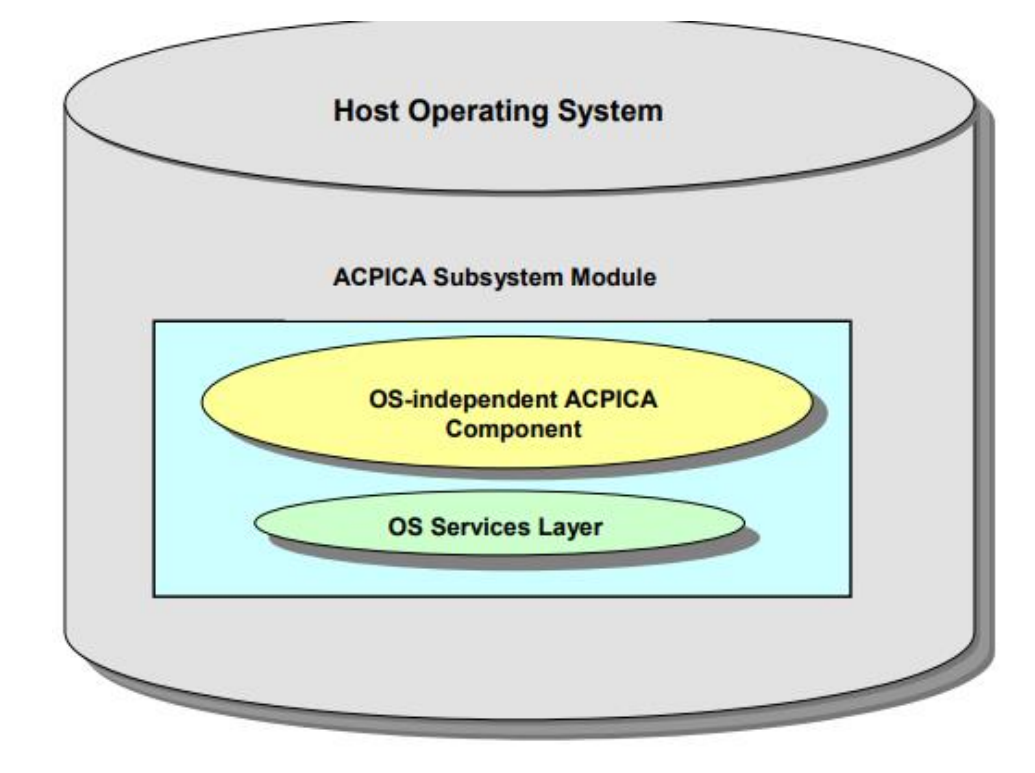
\includegraphics[width=0.7\linewidth]{introduction/acpica-subsystem-architecture}
	\caption{ACPICA Subsystem Architecture}\label{fig:introduction-acpica-subsystem-architecture}
\end{figure}

\subsubsection{ACPICA Subsystem Interaction}
The ACPICA Subsystem implements a set of external interfaces that can be directly called from
the host OS. These Acpi* interfaces provide the actual ACPI services for the host. When operating
system services are required during the servicing of an ACPI request, the Subsystem makes
requests to the host OS indirectly via the fixed AcpiOs* interfaces. The diagram below illustrates
the relationships and interaction between the various architectural elements by showing the flow
of control between them. Note that the OS-independent ACPICA Subsystem never calls the host directly instead it makes calls to the AcpiOs * interfaces in the OSL. This provides the ACPICA
code with OS-independence.

The Interaction between the Architectural Components Is shown in Figure \ref{fig:-introduction-acpi-interaction-between-the-architectural-components}

\begin{figure}[h]
	\centering
	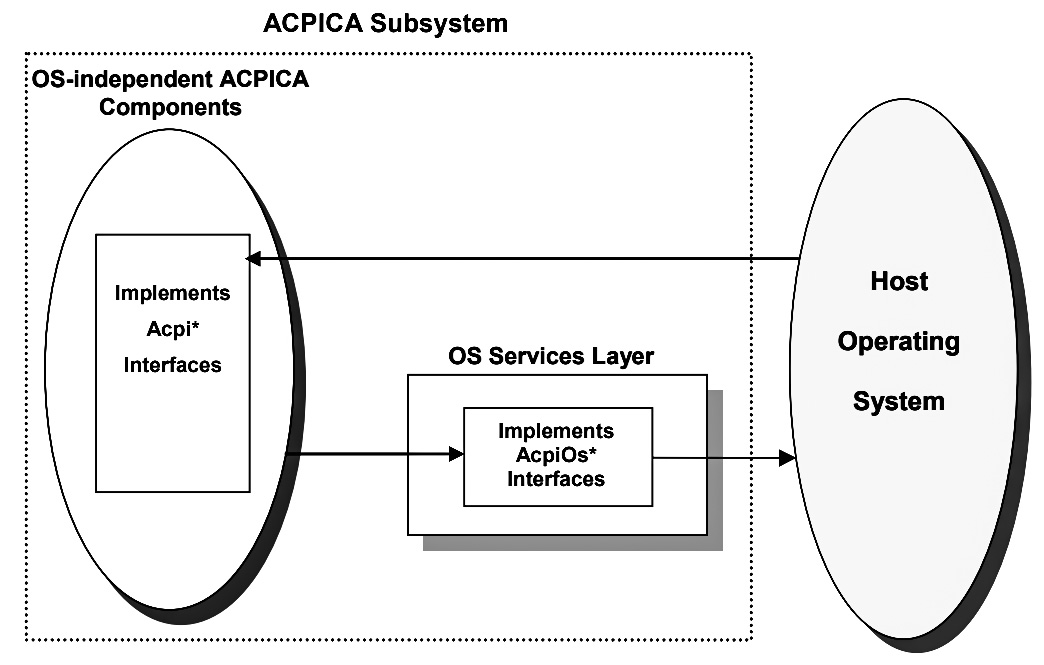
\includegraphics[width=0.7\linewidth]{introduction/acpi-interaction-between-the-architectural-components}
	\caption{Interaction between the Architectural Components}\label{fig:-introduction-acpi-interaction-between-the-architectural-components}
\end{figure}


\subsection{Peripheral Component Interconnect Express (\gls{pcie})}
The \say{Peripheral Component Interconnect (PCI)} architecture has emerged out to be a very thriving beyond even the many more optimistic prospects. Today about every new computer system arrives equipped with at least one PCI slots. Even though there are about to countless PCI slots are shipped globally, there does exists tons of PCI adapter cards which are available to fulfill the all the virtual possible application needs.

This fast growing generation has also raised the demand for many new higher performance interface for input-output communication to support rising technology such as ultra high bandwidth technologies like $ 10-Gb $ Ethernet, $ 10-Gb $ \say{FibreChannel}, $ 12X $ InfiniBand and many more. A regulation which could adapt to carrying out these high performance objectives, while withholding compatibility for previous generation of PCI would beyond any doubt can offer the idealistic solution.

\say{PCI-X 2.0} standard has been developed to meet these objectives. It is capable to serve the uninterrupted performance to feed the nearly all high-bandwidth programs while at the same instance keeping up the full hardware and software backward compatibility for previous \say{PCI} and \say{PCI-X} generations. The PCI-X 2.0 regulation establishes two new grades of speed and performance which are PCI-X 266 and PCI-X 533. These speed grades endeavors bandwidths that are twice and fourfold that of previous generation PCI-X 133 which results to finally supplying bandwidths which are $ 32x $ faster compared to the older version of PCI. It successfully succeeds to bring of additional required performance via time-proven \say{Double Data Rate (DDR)} and \say{Quad Data Rate (QDR)} mechanisms that transmit data at either twice or fourfold the base frequency of clock. As the PCI-X 2.0 conserves too many modules of previous generation PCI it's beneficiary for terrific amount of preceding development job. The OS, device drivers, protocols, connectors, form factor, BIOS, electrical signals, Bus functional modal among many more original PCI modules are all greatly rendered in the new PCI-X 2.0 specification.
Also, many of these modules actually remains untouched in PCI-X 2.0. Due to not having the much of the dissimilarity, it enables development easier because these modules have been already designed and developed with required engineering and familiar to the developers. As a end result, risk is dramatically decreased because the time-to-market became short.

\subsubsection{Functional Description}
The hardware which is used to implement a PCI based system consumes a software interface served by PCI BIOS feature. It has elementary use to generate operations in address spaces specific to PCI (PCI configuration space).

The X86 architecture allows following mode to operate as per PCI BIOS features:
\begin{itemize}
  \item Real mode
  \item Protected mode
    \begin{itemize}
      \item $ 286 $ protected mode $ (16:16) $
      \item $ 386 $ protected mode $ (16:32) $
    \end{itemize}
  \item Flat mode (0:32 protected mode)
\end{itemize}
In the Flat mode, all the segments begun at linear address $ 0 $ and span till the end of the whole $ 4-GB $ address space.

\subsubsection{BUS Performances and Number of Slots Compared}
The several architectures characterized by the PCISIG. Figure \ref{fig:comparison-of-bus-frequency-bandwidth-slots} portrays the development of PCI bus clock frequencies and bandwidths. Its pretty obvious that the increasing the bus frequency does comprise the load in terms of electrical nodes as also to the maximum permissible connectors on a bus at that clock frequencies.

\begin{figure}[!htbp]
	\centering
	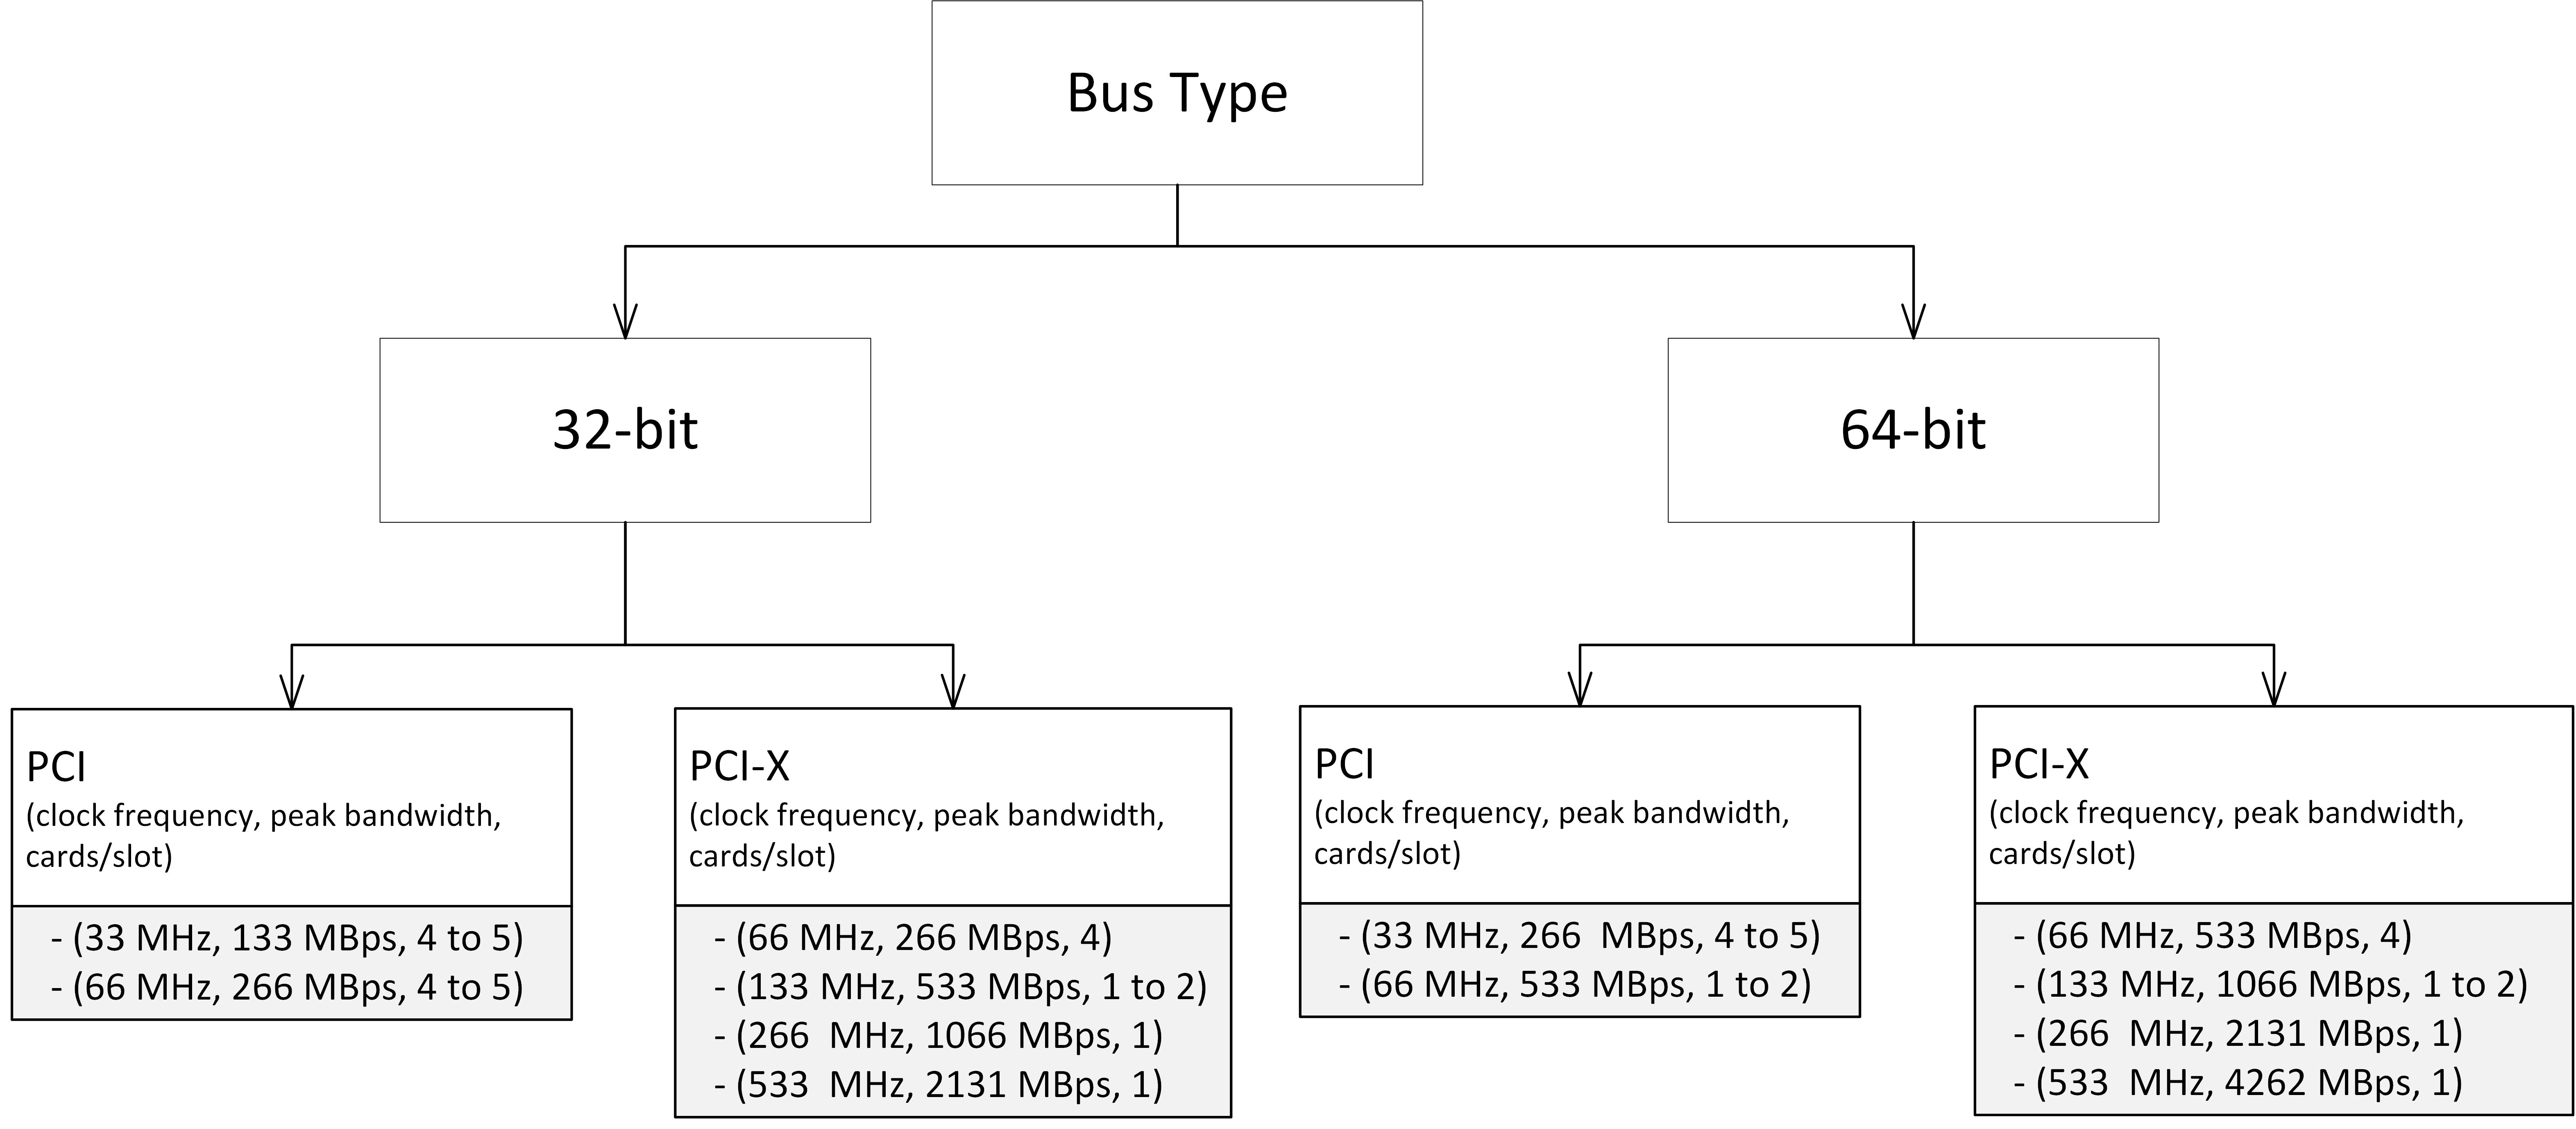
\includegraphics[width=\linewidth]{introduction/comparison-of-bus-frequency-bandwidth-slots}
	\caption{Comparison of Bus Frequency, Bandwidth and Number of Slots}\label{fig:comparison-of-bus-frequency-bandwidth-slots}
\end{figure}

A \say{PCI express (PCIe) Interconnect} is responsible in connecting two PCI devices via PCI link. A PCI link consists if any signal pairs in each direction. These signals ($ x1, x2, x4, x8, x12, x16, x32 $) known as the Lanes. A BIOS designer decides that how many Lanes implementation should be permissible based on the benchmark performance of targeted platform on a given PCI link.

Figure \ref{fig:comparison-of-bus-frequency-bandwidth-slots} portrays the total bandwidth values for various PCI link width.



\subsection{Graphics Controller}
Almost every graphics controllers are merely PCI controllers only. And it is also obvious that the graphics drivers who are responsible to control and manage these graphics controllers are also PCI drivers. Note that even if the most graphics controllers are PCI controllers but even then the graphics controllers can also utilize many of the other buses i.e. USB buses. 

Characterizes of Graphics drivers are listed below:
\begin{itemize}
	\item Follows UEFI Driver Modal
	\item Depending on the driver manged adapter, a graphics driver could be classified as into: a single output adapter and a multiple output adapter.
	\item For each output expected, the graphics driver has to construct child handles.
	\item For some of the output ports and protocols (such as GOP Protocol) the graphics drivers must create child handles.
	\item Graphics drivers are chip-specific because of the requirement to initialize and manage the graphics device.
\end{itemize}
Note that (\gls{ihv}) has privilege for choosing whether to support and implement all the required modules of the UEFI specification. i.e., all modules might not be implemented to support on a specified system configuration which doesn't support all of the services and features understood by the needed modules.

\subsubsection{Graphics Output Protocol (\gls{gop})}
The \say{Graphics Output Protocol \gls{gop}} Driver is member of the driver of UEFI boot time which are responsible for running up the display while the bios is booting. This driver triggers displaying of logo while the bios is booting.

\subsubsection{GOP Overview}
The GOP driver is the successor for video controller of legacy BIOS and sheers the utilization of UEFI pre-boot firmware without the use of CSM. The GOP driver can be $ 32-bit $, $ 64-bit $, or $ IA-64 $ with no binary support. Pre-boot firmware architecture of UEFI which could be either $ 32-bit $ or $ 64-bit $ has to adapt the corresponding GOP driver architecture ($ 32-bit $ or $ 64-bit $). The GOP driver could be one of the boot mode: \say{fastboot} (for specific platform optimized mode to speedup the boot time) or \say{generic} (the normal boot process).

\subsubsection{GOP DRIVER}
The EFI specification characterizes the \say{Universal Graphic Adapter (UGA)} protocol to provide graphics which could be device-independent. However, Specification of UEFI eliminated the inclusion of UGA and replaced it with it's successor \gls{gop} so that VGA hardware dependencies can be removed.

\subsubsection{GOP Integration}
The platform firmware must meet the following requirements for GOP Driver integration:
\begin{itemize}
	\item Platform firmware must be compliant to UEFI 2.1 or later.
	\item Platform must enumerate and initialize the graphics device.
	\item Platform must allocate enough graphics frame buffer memory required to support the native mode resolution of the integrated display.
	\item The platform must produce the standard \verb|EFI_PCI_IO_PROTOCOL| and as well as the \verb|EFI_DEVICE_PATH_PROTOCOL| on the graphics device handle. Additionally, the platform must produce \verb|PLATFORM_GOP_POLICY_PROTOCOL|.
	\item The platform firmware must not launch the legacy Video BIOS.
\end{itemize}

The GOP Driver solution comprises the following files shown in Table \ref{table:gop-driver-files} GOP driver files.

\begin{table}
	\centering
	\renewcommand\arraystretch{2}
	\caption{\gls{gop} Driver files}\label{table:gop-driver-files}
	\begin{tabular}{l | p{5cm} | p{5cm}}
		File Name & Description & Format
		\\ \hline \hline
		\verb|GopDriver.efi| & The \gls{gop} driver binary & Uncompressed PE/COFF image
		\\ \hline
		\verb|Vbt.bin| & Contains Video BIOS Table (VBT) data & Raw Binary
		\\ \hline
		\verb|Vbt.bsf| & BMP script file. Required for modifying Vbt.bin using BMP tool & Text
		\\ \hline
	\end{tabular}
\end{table}

Customize the VBT data file\verb| Vbt.bin| as per platform requirements and the corresponding BSF file. Integrate \verb|Vbt.bin| and \verb|GopDriver.efi| files into the platform firmware image. The process of accomplishing this step is determined by the platform implementer, specific to the platform firmware implementation.

